\section{Preliminary comments}

We note that the formulation of \acrshort{iot}
in~\cite{schoellhammer2004lightweight} relies on the intersection of
\emph{convex cones} in dimension $n+1$. For $n=1$, it corresponds to the
intersection of triangles, which can efficiently be computed by maintaining
boundary lines, as detailed previously Section~\ref{sec:ltc}. In higher
dimension, however, cone intersections are not so straightforward to compute,
due to the fact that the intersection between cones may not be a cone.

To address this issue, we formulate \acrshort{iot} as an intersection test
between \emph{n-balls}, that is, segments for $n=1$, disks for $n=2$, etc.
N-balls are defined from the \emph{norm} used in the vector space of data
points. For $n=1$, the choice of the norm does not really matter, as all p-norms
and the infinity norm are identical. In dimension $n$, however, norm selection
will be critical.

\section{Algebraic formulation of LTC}

\subsection{Definitions}

%% notation
Above all, we give the notation of \acrshort{ltc} in the
following: The algorithm receives a stream of data points $x_i$ at times $t_i$
($i \in \mathbb{N}$), and it transmits a stream of data points $\xi_i$ at times
$\tau_i$ ($i \in \mathbb{N}$). To simplify the notations, we assume that:
\begin{equation}
\forall k \in \mathbb{N}, \  \exists ! i \in \mathbb{N} \  \tau_k = t_i
\end{equation}
That is, transmission times coincide with reception times.
We define the \emph{shifted received points} as follows:
\begin{equation}
\label{eq:ltc-2}
\forall k \in \mathbb{N}\ , \forall j \in \mathbb{N^*},\ (u^k_j, y^k_j) = (t_{i+j}, x_{i+j}), 
\end{equation}
where $i$ is such that $t_i = \tau_k$ and:
\begin{equation}
\label{eq:ltc-3}
\forall k \in \mathbb{N},\  (u^k_0, y^k_0) = (\tau_k, \xi_k).
\end{equation}
This definition is such that $y^k_j$ is the $j^{th}$ data point received
after the $k^{th}$ transmission and $u^k_j$ is the corresponding time-stamp.
Figure~\ref{fig:ltc-notation} illustrates the notations and algorithm.

Using these notations and details in Section~\ref{sec:ltc}, the original
\acrshort{ltc} algorithm can be written as in Algorithm~\ref{algo:ltc-notation}.
For readability, we assume that access to data points is blocking, i.e., the
program will wait until the points are available. We also assume that the
content of variable \texttt{tr} is transmitted after each assignment of this
variable. Function \texttt{line}, omitted for brevity, returns the ordinate at
abscissa $x$ (1st argument) of the line defined by the points in its 2nd and 3rd
arguments.

\begin{figure}[H]
\centering
\includegraphics[width=0.8\columnwidth]{./figures/ltc.pdf}
\caption{Illustration of the \acrshort{ltc} algorithm. Blue 
dots are received points, red dots are transmitted points. Dashed lines 
represent the high and low lines when a point is 
transmitted.\vspace*{-0.3cm}}
\label{fig:ltc-notation}
\end{figure}

\begin{algorithm}
\begin{algorithmic}[1]
\Input
   \Desc{$(u^k_j, y^k_j)$}{$\quad \quad $Received data stream}
   \Desc{$\epsilon$}{$\quad \quad$Error bound}
\EndInput
\Output
   \Desc{tr}{Transmitted points}
\EndOutput
\State tr = $(u^0_0, y^0_0)$ \Comment{Last transmitted point}
\State k = 0 ; j = 1
\State (lp, hp) = ($y^0_1 - \epsilon$, $y^0_1 + \epsilon$) \Comment{Low and high points}

\While{True} \Comment{Process received points as they come}
    \State j += 1
    \State new\_lp = max($y^k_j-\epsilon$, line($u^k_j$, tr, ($u^k_{j-1}$, lp)))
    \State new\_hp = min($y^k_j+\epsilon$, line($u^k_j$, tr, ($u^k_{j-1}$, hp)))
    \If{new\_lp $\leq$ new\_hp} \Comment{Keep compressing}
        \State (lp, hp) = (new\_lp, new\_hp)
    \Else
        \State tr = $(u^k_{j-1}, (lp+hp)/2)$
        \Comment{Transmit point}
        \State k += 1
        \State j = 1
        \State (lp, hp) = ($y^k_j-\epsilon$, $y^k_j+\epsilon$)
    \EndIf
\EndWhile
\end{algorithmic}
\caption{Original \acrshort{ltc} algorithm, adapted from~\cite{schoellhammer2004lightweight}.}
\label{algo:ltc-notation}
\end{algorithm}


%% define
According to equations~\eqref{eq:ltc-2} and~\eqref{eq:ltc-3}, let $(u_0^k,
y_0^k) \in \mathbb{R}^{n+1}$ be the latest transmitted point. For convenience,
all the subsequent points will be expressed in the orthogonal space with origin
$(\tau_k, \xi_k)$ through equation~\eqref{eq:ltc-3}. We denote by $(v_j, z_j)_{j
\in \llbracket 0, m \rrbracket}$ such points:
\begin{equation}
\forall j \leq m,\  (v_j, z_j) = (u_j^k - \tau_k, y_j^k - \xi_k)
\end{equation}
Let $\mathcal{B}_j$ be the ball of $\mathbb{R}^n$ of centre $\frac{v_1}{v_j}z_j$
and radius $\frac{v_1}{v_j}\epsilon$:
\begin{equation}
\mathcal{B}_j = \left\{ z \in \mathbb{R}^n,\norm{z-\frac{v_1}{v_j}z_j} \leq\frac{v_1}{v_j}\epsilon \right\}
\end{equation}
Note that $v_1$ is defined as soon as one point is received after the last
transmission.

\subsection{\acrshort{ltc} property}
\label{sec:ltc-property}

We define the \emph{\acrshort{ltc} property} as follows:
\begin{equation}
\exists z \in \mathbb{R}^n, \ \forall j \in \llbracket 1, m \rrbracket, \norm{\frac{v_j}{v_1}z-z_j} \leq
\epsilon.
\end{equation}
The original \acrshort{ltc} algorithm ensures that the \acrshort{ltc} property
is verified between each transmissions. Indeed, all the data points $z$ such
that $(v_1, z)$ is between the high line and the low line verify the property.
Line 13 in Algorithm~\ref{algo:ltc-notation} guarantees that such a point
exists.

The \acrshort{ltc} property can be re-written as follows:
\begin{equation}
\exists z \in \mathbb{R}^n, \ \forall j \in \llbracket 1, m \rrbracket, \norm{z-\frac{v_1}{v_j}z_j} \leq
\frac{v_1}{v_j}\epsilon
\end{equation}
that is:
\begin{equation}
\bigcap_{j=1}^m \mathcal{B}_j \neq \text{\O}
\label{eq:ltc-property}
\end{equation}
Note that $(\mathcal{B}_j)_{j \in \llbracket 1, m \rrbracket}$ is a sequence
of n-balls of strictly decreasing radius, since $v_j > v_1$.

\section{Algorithm}

The \acrshort{ltc} algorithm generalized to dimension $n$ tests that the
\acrshort{ltc} property in Equation~\ref{eq:ltc-property} is verified after each
reception of a data point. It is written in Algorithm~\ref{algo:general-ltc}.
\begin{algorithm}
\begin{algorithmic}[1]
\Input
   \Desc{$(u^k_j, y^k_j)$}{$\quad \quad $Received data stream}
   \Desc{$\epsilon$}{$\quad \quad$Error bound}
\EndInput
\Output
   \Desc{tr}{Transmitted points}
\EndOutput

\State tr = ($\tau, \xi$) = ($u^0_0, y^0_0$) \Comment{Last transmitted point}
\State k = 0 ; j = 0
\While{True}
    \State j += 1
    \State ($v_j, z_j$) = ($u_j^k - \tau, y_j^k - \xi$)
    \If{$\bigcap_{l=1}^j{\mathcal{B}_l} = \text{\O}$}
        \State Pick $z$ in $\bigcap_{l=1}^{j-1}{\mathcal{B}_l}$ \Comment{Transmit point}
        \State tr = ($\tau$, $\xi$) = ($u^k_{j-1}, z$)
        \State k += 1
        \State j = 1
    \EndIf
\EndWhile
\end{algorithmic}
\caption{Generalized LTC.}
\label{algo:general-ltc}
\end{algorithm}

\section{Intersections of n-balls}

Although Algorithm~\ref{algo:general-ltc} looks simple, one should not overlook
the fact that there is no good general algorithm to test whether a set of
n-balls intersect. The best general algorithm we could find so far relies on
Helly's theorem which is formulated as follows~\cite{helly1923mengen}:
\begin{theorem}
Let $\left\{ X_i \right\}_{i \in \llbracket 1, m \rrbracket}$ be a collection of
convex subsets of $\mathbb{R}^n$. If the intersection of every $n+1$ subsets is
non-empty, then the whole collection has an non-empty intersection.
\end{theorem}
% \noindent This theorem leads to an algorithm of complexity ${m \choose n+1}$
% which is not usable in resource-constrained environments such as connected
% objects.
\noindent This theorem leads to an algorithm of complexity ${\binom{m}{n+1}}$
which is not usable in resource-constrained environments such as connected
objects.

The only feasible algorithm that we found is norm-specific. It
maintains a representation of the intersection
$\bigcap_{j=1}^{m}{\mathcal{B}_j}$ that is updated at every iteration.
The intersection tests can then be done in constant time. However,
updating the representation of the intersection may be costly
depending on the norm used. For the infinity norm, the representation
is a rectangular cuboid which is straightforward to update by
intersection with an n-ball.
For the Euclidean norm, the representation is an arbitrary volume,
which is more costly to maintain.

\section{Effect of the norm}
\label{sec:effect-norm}

As mentioned before, norm selection in $\mathbb{R}^n$ has a critical impact on
the compression error and ratio. To appreciate this effect, let us compare the
infinity norm and the Euclidean norm in dimension 2. By comparing the unit disk
to a square of side 2, we obtain that the compression ratio of a random stream
would be $\frac{4}{\pi}$ times larger with the infinity norm than with the
Euclidean norm (see Figure~\ref{fig:norm-comparison-2D}). In 3D, this ratio
would be $\frac{6}{\pi}$. Unsurprisingly, the infinity norm is more tolerant
than the Euclidean norm.

It should also be noted that using the infinity norm in $\mathbb{R}^n$ boils
down to the use of the 1D LTC algorithm independently in each dimension, since
a data point will be transmitted as soon as the linear approximation doesn't
hold in any of the dimensions. For the Euclidean norm, however, the
multidimensional and multiple unidimensional versions are different: the
multiple unidimensional version behaves as the infinity norm, but the
multidimensional version is more stringent, leading to a reduced compression
rate and error.

To choose between the multidimensional implementation and multiple
unidimensional ones, we recommend to check whether the desired error bound is
expressed independently for every sensor, or as an aggregate error between them.
The multidimensional version is more appropriate for multidimensional sensors,
for instance 3D accelerometers or 3D gyroscopes, and the multiple unidimensional
version is more suitable for multiple independent sensors, for instance a
temperature and a pressure sensor.

%~ For instance, in case of a 3D accelerometer, if the error 
%~ is expressed simply as 
%~ ``10~mg", then the multidimensional version should be chosen because it 
%~ will guarantee that the norm of the 3D acceleration vector will be 
%~ reconstructed with an error less than 10~mg. Conversely, if the error is 
%~ specified as ``10~mg in x, 
%~ 10~mg in y and 10~mg in z", then the multiple unidimensional version 
%~ should be used.

\begin{figure}
    \centering
    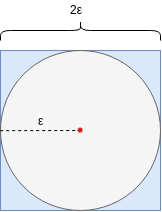
\includegraphics[width=0.3\textwidth]{figures/2D_Comparison.png}
    \caption{Comparison of compression ratio between Infinity norm and Euclidean norm in 2D}
    \label{fig:norm-comparison-2D}
\end{figure}
